\documentclass[12pt]{ociamthesis}  % default square logo 
%\documentclass[12pt,beltcrest]{ociamthesis} % use old belt crest logo
%\documentclass[12pt,shieldcrest]{ociamthesis} % use older shield crest logo

%load any additional packages
\usepackage{amssymb}

%code environment in appendix
%check https://www.sharelatex.com/learn/Code_listing for documentation
\usepackage[utf8]{inputenc}


\usepackage{marvosym}
 
\usepackage{listings}
\usepackage{color}

\usepackage{array}

\usepackage{booktabs}
\usepackage{multirow}
\usepackage{siunitx}
\usepackage{bigdelim}

\usepackage{eurosym}


\usepackage{enumerate}
\usepackage{amsmath}
\usepackage{bbm}

\usepackage{verbatim}

%\usepackage{url} % hyperref works too
%\urlstyle{same}  % (sf also works, for something more subtle than tt)

\usepackage{graphicx}
\usepackage{caption}

\widowpenalty10000
\clubpenalty10000

\usepackage[table]{xcolor}
\usepackage[color=green]{todonotes}

\usepackage{ltxtable}
\usepackage{float}


\usepackage[round]{natbib}

\usepackage{pgfplots}
\usepgfplotslibrary{external}
\usepgfplotslibrary{patchplots}
\usepgfplotslibrary{units}
\usetikzlibrary{pgfplots.statistics}
\usepgfplotslibrary{dateplot}
\usepackage{pgfcalendar}
\usepackage{filecontents}

\usepackage{url} % hyperref works too
\PassOptionsToPackage{hyphens}{url}
\g@addto@macro{\UrlBreaks}{\UrlOrds}
%\usepackage[anythingbreaks]{breakurl}

\urlstyle{same}  % (sf also works, for something more subtle than tt)

\pgfplotsset{
  xpercent/.style={
    change x base,
    x SI prefix = centi,
    xticklabel  = {\pgfmathprintnumber{\tick}\,\%},
  },
  ypercent/.style={
    change y base,
    y SI prefix = centi,
    yticklabel  = {\pgfmathprintnumber{\tick}\,\%},
  },
  zpercent/.style={
    change z base,
    z SI prefix = centi,
    zticklabel  = {\pgfmathprintnumber{\tick}\,\%},
  },
}

\pgfplotsset{compat=1.12}

\pgfplotsset{compat=1.12,
  colormap/viridis/.style={
    colormap={viridis}{
      rgb=(0.26700401,  0.00487433,  0.32941519)
      rgb=(0.26851048,  0.00960483,  0.33542652)
      rgb=(0.26994384,  0.01462494,  0.34137895)
      rgb=(0.27130489,  0.01994186,  0.34726862)
      rgb=(0.27259384,  0.02556309,  0.35309303)
      rgb=(0.27380934,  0.03149748,  0.35885256)
      rgb=(0.27495242,  0.03775181,  0.36454323)
      rgb=(0.27602238,  0.04416723,  0.37016418)
      rgb=(0.2770184 ,  0.05034437,  0.37571452)
      rgb=(0.27794143,  0.05632444,  0.38119074)
      rgb=(0.27879067,  0.06214536,  0.38659204)
      rgb=(0.2795655 ,  0.06783587,  0.39191723)
      rgb=(0.28026658,  0.07341724,  0.39716349)
      rgb=(0.28089358,  0.07890703,  0.40232944)
      rgb=(0.28144581,  0.0843197 ,  0.40741404)
      rgb=(0.28192358,  0.08966622,  0.41241521)
      rgb=(0.28232739,  0.09495545,  0.41733086)
      rgb=(0.28265633,  0.10019576,  0.42216032)
      rgb=(0.28291049,  0.10539345,  0.42690202)
      rgb=(0.28309095,  0.11055307,  0.43155375)
      rgb=(0.28319704,  0.11567966,  0.43611482)
      rgb=(0.28322882,  0.12077701,  0.44058404)
      rgb=(0.28318684,  0.12584799,  0.44496   )
      rgb=(0.283072  ,  0.13089477,  0.44924127)
      rgb=(0.28288389,  0.13592005,  0.45342734)
      rgb=(0.28262297,  0.14092556,  0.45751726)
      rgb=(0.28229037,  0.14591233,  0.46150995)
      rgb=(0.28188676,  0.15088147,  0.46540474)
      rgb=(0.28141228,  0.15583425,  0.46920128)
      rgb=(0.28086773,  0.16077132,  0.47289909)
      rgb=(0.28025468,  0.16569272,  0.47649762)
      rgb=(0.27957399,  0.17059884,  0.47999675)
      rgb=(0.27882618,  0.1754902 ,  0.48339654)
      rgb=(0.27801236,  0.18036684,  0.48669702)
      rgb=(0.27713437,  0.18522836,  0.48989831)
      rgb=(0.27619376,  0.19007447,  0.49300074)
      rgb=(0.27519116,  0.1949054 ,  0.49600488)
      rgb=(0.27412802,  0.19972086,  0.49891131)
      rgb=(0.27300596,  0.20452049,  0.50172076)
      rgb=(0.27182812,  0.20930306,  0.50443413)
      rgb=(0.27059473,  0.21406899,  0.50705243)
      rgb=(0.26930756,  0.21881782,  0.50957678)
      rgb=(0.26796846,  0.22354911,  0.5120084 )
      rgb=(0.26657984,  0.2282621 ,  0.5143487 )
      rgb=(0.2651445 ,  0.23295593,  0.5165993 )
      rgb=(0.2636632 ,  0.23763078,  0.51876163)
      rgb=(0.26213801,  0.24228619,  0.52083736)
      rgb=(0.26057103,  0.2469217 ,  0.52282822)
      rgb=(0.25896451,  0.25153685,  0.52473609)
      rgb=(0.25732244,  0.2561304 ,  0.52656332)
      rgb=(0.25564519,  0.26070284,  0.52831152)
      rgb=(0.25393498,  0.26525384,  0.52998273)
      rgb=(0.25219404,  0.26978306,  0.53157905)
      rgb=(0.25042462,  0.27429024,  0.53310261)
      rgb=(0.24862899,  0.27877509,  0.53455561)
      rgb=(0.2468114 ,  0.28323662,  0.53594093)
      rgb=(0.24497208,  0.28767547,  0.53726018)
      rgb=(0.24311324,  0.29209154,  0.53851561)
      rgb=(0.24123708,  0.29648471,  0.53970946)
      rgb=(0.23934575,  0.30085494,  0.54084398)
      rgb=(0.23744138,  0.30520222,  0.5419214 )
      rgb=(0.23552606,  0.30952657,  0.54294396)
      rgb=(0.23360277,  0.31382773,  0.54391424)
      rgb=(0.2316735 ,  0.3181058 ,  0.54483444)
      rgb=(0.22973926,  0.32236127,  0.54570633)
      rgb=(0.22780192,  0.32659432,  0.546532  )
      rgb=(0.2258633 ,  0.33080515,  0.54731353)
      rgb=(0.22392515,  0.334994  ,  0.54805291)
      rgb=(0.22198915,  0.33916114,  0.54875211)
      rgb=(0.22005691,  0.34330688,  0.54941304)
      rgb=(0.21812995,  0.34743154,  0.55003755)
      rgb=(0.21620971,  0.35153548,  0.55062743)
      rgb=(0.21429757,  0.35561907,  0.5511844 )
      rgb=(0.21239477,  0.35968273,  0.55171011)
      rgb=(0.2105031 ,  0.36372671,  0.55220646)
      rgb=(0.20862342,  0.36775151,  0.55267486)
      rgb=(0.20675628,  0.37175775,  0.55311653)
      rgb=(0.20490257,  0.37574589,  0.55353282)
      rgb=(0.20306309,  0.37971644,  0.55392505)
      rgb=(0.20123854,  0.38366989,  0.55429441)
      rgb=(0.1994295 ,  0.38760678,  0.55464205)
      rgb=(0.1976365 ,  0.39152762,  0.55496905)
      rgb=(0.19585993,  0.39543297,  0.55527637)
      rgb=(0.19410009,  0.39932336,  0.55556494)
      rgb=(0.19235719,  0.40319934,  0.55583559)
      rgb=(0.19063135,  0.40706148,  0.55608907)
      rgb=(0.18892259,  0.41091033,  0.55632606)
      rgb=(0.18723083,  0.41474645,  0.55654717)
      rgb=(0.18555593,  0.4185704 ,  0.55675292)
      rgb=(0.18389763,  0.42238275,  0.55694377)
      rgb=(0.18225561,  0.42618405,  0.5571201 )
      rgb=(0.18062949,  0.42997486,  0.55728221)
      rgb=(0.17901879,  0.43375572,  0.55743035)
      rgb=(0.17742298,  0.4375272 ,  0.55756466)
      rgb=(0.17584148,  0.44128981,  0.55768526)
      rgb=(0.17427363,  0.4450441 ,  0.55779216)
      rgb=(0.17271876,  0.4487906 ,  0.55788532)
      rgb=(0.17117615,  0.4525298 ,  0.55796464)
      rgb=(0.16964573,  0.45626209,  0.55803034)
      rgb=(0.16812641,  0.45998802,  0.55808199)
      rgb=(0.1666171 ,  0.46370813,  0.55811913)
      rgb=(0.16511703,  0.4674229 ,  0.55814141)
      rgb=(0.16362543,  0.47113278,  0.55814842)
      rgb=(0.16214155,  0.47483821,  0.55813967)
      rgb=(0.16066467,  0.47853961,  0.55811466)
      rgb=(0.15919413,  0.4822374 ,  0.5580728 )
      rgb=(0.15772933,  0.48593197,  0.55801347)
      rgb=(0.15626973,  0.4896237 ,  0.557936  )
      rgb=(0.15481488,  0.49331293,  0.55783967)
      rgb=(0.15336445,  0.49700003,  0.55772371)
      rgb=(0.1519182 ,  0.50068529,  0.55758733)
      rgb=(0.15047605,  0.50436904,  0.55742968)
      rgb=(0.14903918,  0.50805136,  0.5572505 )
      rgb=(0.14760731,  0.51173263,  0.55704861)
      rgb=(0.14618026,  0.51541316,  0.55682271)
      rgb=(0.14475863,  0.51909319,  0.55657181)
      rgb=(0.14334327,  0.52277292,  0.55629491)
      rgb=(0.14193527,  0.52645254,  0.55599097)
      rgb=(0.14053599,  0.53013219,  0.55565893)
      rgb=(0.13914708,  0.53381201,  0.55529773)
      rgb=(0.13777048,  0.53749213,  0.55490625)
      rgb=(0.1364085 ,  0.54117264,  0.55448339)
      rgb=(0.13506561,  0.54485335,  0.55402906)
      rgb=(0.13374299,  0.54853458,  0.55354108)
      rgb=(0.13244401,  0.55221637,  0.55301828)
      rgb=(0.13117249,  0.55589872,  0.55245948)
      rgb=(0.1299327 ,  0.55958162,  0.55186354)
      rgb=(0.12872938,  0.56326503,  0.55122927)
      rgb=(0.12756771,  0.56694891,  0.55055551)
      rgb=(0.12645338,  0.57063316,  0.5498411 )
      rgb=(0.12539383,  0.57431754,  0.54908564)
      rgb=(0.12439474,  0.57800205,  0.5482874 )
      rgb=(0.12346281,  0.58168661,  0.54744498)
      rgb=(0.12260562,  0.58537105,  0.54655722)
      rgb=(0.12183122,  0.58905521,  0.54562298)
      rgb=(0.12114807,  0.59273889,  0.54464114)
      rgb=(0.12056501,  0.59642187,  0.54361058)
      rgb=(0.12009154,  0.60010387,  0.54253043)
      rgb=(0.11973756,  0.60378459,  0.54139999)
      rgb=(0.11951163,  0.60746388,  0.54021751)
      rgb=(0.11942341,  0.61114146,  0.53898192)
      rgb=(0.11948255,  0.61481702,  0.53769219)
      rgb=(0.11969858,  0.61849025,  0.53634733)
      rgb=(0.12008079,  0.62216081,  0.53494633)
      rgb=(0.12063824,  0.62582833,  0.53348834)
      rgb=(0.12137972,  0.62949242,  0.53197275)
      rgb=(0.12231244,  0.63315277,  0.53039808)
      rgb=(0.12344358,  0.63680899,  0.52876343)
      rgb=(0.12477953,  0.64046069,  0.52706792)
      rgb=(0.12632581,  0.64410744,  0.52531069)
      rgb=(0.12808703,  0.64774881,  0.52349092)
      rgb=(0.13006688,  0.65138436,  0.52160791)
      rgb=(0.13226797,  0.65501363,  0.51966086)
      rgb=(0.13469183,  0.65863619,  0.5176488 )
      rgb=(0.13733921,  0.66225157,  0.51557101)
      rgb=(0.14020991,  0.66585927,  0.5134268 )
      rgb=(0.14330291,  0.66945881,  0.51121549)
      rgb=(0.1466164 ,  0.67304968,  0.50893644)
      rgb=(0.15014782,  0.67663139,  0.5065889 )
      rgb=(0.15389405,  0.68020343,  0.50417217)
      rgb=(0.15785146,  0.68376525,  0.50168574)
      rgb=(0.16201598,  0.68731632,  0.49912906)
      rgb=(0.1663832 ,  0.69085611,  0.49650163)
      rgb=(0.1709484 ,  0.69438405,  0.49380294)
      rgb=(0.17570671,  0.6978996 ,  0.49103252)
      rgb=(0.18065314,  0.70140222,  0.48818938)
      rgb=(0.18578266,  0.70489133,  0.48527326)
      rgb=(0.19109018,  0.70836635,  0.48228395)
      rgb=(0.19657063,  0.71182668,  0.47922108)
      rgb=(0.20221902,  0.71527175,  0.47608431)
      rgb=(0.20803045,  0.71870095,  0.4728733 )
      rgb=(0.21400015,  0.72211371,  0.46958774)
      rgb=(0.22012381,  0.72550945,  0.46622638)
      rgb=(0.2263969 ,  0.72888753,  0.46278934)
      rgb=(0.23281498,  0.73224735,  0.45927675)
      rgb=(0.2393739 ,  0.73558828,  0.45568838)
      rgb=(0.24606968,  0.73890972,  0.45202405)
      rgb=(0.25289851,  0.74221104,  0.44828355)
      rgb=(0.25985676,  0.74549162,  0.44446673)
      rgb=(0.26694127,  0.74875084,  0.44057284)
      rgb=(0.27414922,  0.75198807,  0.4366009 )
      rgb=(0.28147681,  0.75520266,  0.43255207)
      rgb=(0.28892102,  0.75839399,  0.42842626)
      rgb=(0.29647899,  0.76156142,  0.42422341)
      rgb=(0.30414796,  0.76470433,  0.41994346)
      rgb=(0.31192534,  0.76782207,  0.41558638)
      rgb=(0.3198086 ,  0.77091403,  0.41115215)
      rgb=(0.3277958 ,  0.77397953,  0.40664011)
      rgb=(0.33588539,  0.7770179 ,  0.40204917)
      rgb=(0.34407411,  0.78002855,  0.39738103)
      rgb=(0.35235985,  0.78301086,  0.39263579)
      rgb=(0.36074053,  0.78596419,  0.38781353)
      rgb=(0.3692142 ,  0.78888793,  0.38291438)
      rgb=(0.37777892,  0.79178146,  0.3779385 )
      rgb=(0.38643282,  0.79464415,  0.37288606)
      rgb=(0.39517408,  0.79747541,  0.36775726)
      rgb=(0.40400101,  0.80027461,  0.36255223)
      rgb=(0.4129135 ,  0.80304099,  0.35726893)
      rgb=(0.42190813,  0.80577412,  0.35191009)
      rgb=(0.43098317,  0.80847343,  0.34647607)
      rgb=(0.44013691,  0.81113836,  0.3409673 )
      rgb=(0.44936763,  0.81376835,  0.33538426)
      rgb=(0.45867362,  0.81636288,  0.32972749)
      rgb=(0.46805314,  0.81892143,  0.32399761)
      rgb=(0.47750446,  0.82144351,  0.31819529)
      rgb=(0.4870258 ,  0.82392862,  0.31232133)
      rgb=(0.49661536,  0.82637633,  0.30637661)
      rgb=(0.5062713 ,  0.82878621,  0.30036211)
      rgb=(0.51599182,  0.83115784,  0.29427888)
      rgb=(0.52577622,  0.83349064,  0.2881265 )
      rgb=(0.5356211 ,  0.83578452,  0.28190832)
      rgb=(0.5455244 ,  0.83803918,  0.27562602)
      rgb=(0.55548397,  0.84025437,  0.26928147)
      rgb=(0.5654976 ,  0.8424299 ,  0.26287683)
      rgb=(0.57556297,  0.84456561,  0.25641457)
      rgb=(0.58567772,  0.84666139,  0.24989748)
      rgb=(0.59583934,  0.84871722,  0.24332878)
      rgb=(0.60604528,  0.8507331 ,  0.23671214)
      rgb=(0.61629283,  0.85270912,  0.23005179)
      rgb=(0.62657923,  0.85464543,  0.22335258)
      rgb=(0.63690157,  0.85654226,  0.21662012)
      rgb=(0.64725685,  0.85839991,  0.20986086)
      rgb=(0.65764197,  0.86021878,  0.20308229)
      rgb=(0.66805369,  0.86199932,  0.19629307)
      rgb=(0.67848868,  0.86374211,  0.18950326)
      rgb=(0.68894351,  0.86544779,  0.18272455)
      rgb=(0.69941463,  0.86711711,  0.17597055)
      rgb=(0.70989842,  0.86875092,  0.16925712)
      rgb=(0.72039115,  0.87035015,  0.16260273)
      rgb=(0.73088902,  0.87191584,  0.15602894)
      rgb=(0.74138803,  0.87344918,  0.14956101)
      rgb=(0.75188414,  0.87495143,  0.14322828)
      rgb=(0.76237342,  0.87642392,  0.13706449)
      rgb=(0.77285183,  0.87786808,  0.13110864)
      rgb=(0.78331535,  0.87928545,  0.12540538)
      rgb=(0.79375994,  0.88067763,  0.12000532)
      rgb=(0.80418159,  0.88204632,  0.11496505)
      rgb=(0.81457634,  0.88339329,  0.11034678)
      rgb=(0.82494028,  0.88472036,  0.10621724)
      rgb=(0.83526959,  0.88602943,  0.1026459 )
      rgb=(0.84556056,  0.88732243,  0.09970219)
      rgb=(0.8558096 ,  0.88860134,  0.09745186)
      rgb=(0.86601325,  0.88986815,  0.09595277)
      rgb=(0.87616824,  0.89112487,  0.09525046)
      rgb=(0.88627146,  0.89237353,  0.09537439)
      rgb=(0.89632002,  0.89361614,  0.09633538)
      rgb=(0.90631121,  0.89485467,  0.09812496)
      rgb=(0.91624212,  0.89609127,  0.1007168 )
      rgb=(0.92610579,  0.89732977,  0.10407067)
      rgb=(0.93590444,  0.8985704 ,  0.10813094)
      rgb=(0.94563626,  0.899815  ,  0.11283773)
      rgb=(0.95529972,  0.90106534,  0.11812832)
      rgb=(0.96489353,  0.90232311,  0.12394051)
      rgb=(0.97441665,  0.90358991,  0.13021494)
      rgb=(0.98386829,  0.90486726,  0.13689671)
      rgb=(0.99324789,  0.90615657,  0.1439362 )
    }
  }
}

\definecolor{barlecker}{rgb}{0.2795655 ,  0.06783587,  0.39191723}
 
\definecolor{codegreen}{rgb}{0,0.6,0}
\definecolor{codegray}{rgb}{0.5,0.5,0.5}
\definecolor{codepurple}{rgb}{0.58,0,0.82}
\definecolor{backcolour}{rgb}{0.95,0.95,0.92}
 
\lstdefinestyle{mystyle}{
    backgroundcolor=\color{backcolour},   
    commentstyle=\color{codegreen},
    keywordstyle=\color{black},
    numberstyle=\tiny\color{magenta},
    stringstyle=\color{codepurple},
    basicstyle=\footnotesize,
    breakatwhitespace=false,         
    breaklines=true,                 
    captionpos=b,                    
    keepspaces=true,                 
    numbers=left,                    
    numbersep=5pt,                  
    showspaces=false,                
    showstringspaces=false,
    showtabs=false,                  
    tabsize=2
}

\setlength\parindent{0pt}

\lstset{style=mystyle}

%input macros (i.e. write your own macros file called mymacros.tex 
%and uncomment the next line)
%\include{mymacros}

\title{Valuation of Contingent Convertibles with Derivatives}   %note \\[1ex] is a line break in the title
\author{Nicolay Schmitt}             %your name
\college{}  %your college

%\renewcommand{\submittedtext}{change the default text here if needed}
\degree{Master of Science in Finance}     %the degree
\degreedate{August 2016}         %the degree date

%end the preamble and start the document
\begin{document}
\bibliographystyle{plainnat}  %use the plain bibliography style

%this baselineskip gives sufficient line spacing for an examiner to easily
%markup the thesis with comments
\baselineskip=18pt plus1pt

%set the number of sectioning levels that get number and appear in the contents
%\setcounter{secnumdepth}{1}
\setcounter{tocdepth}{1}

\maketitle                  % create a title page from the preamble info
\centerline{}
\centerline{}
\section*{\hfil Valuation of Contingent \hfil}
\section*{\hfil Convertibles with Derivatives \hfil}
\vfill
\vfill
\centerline{Master's Thesis}
\centerline{at Frankfurt School of Finance and Management}
\vfill
\vfill
\centerline{Supervised by}
\centerline{Prof. Dr. Uwe Wystup}
\centerline{Prof. Dr. Thomas Heidorn}
\vfill
\vfill
\centerline{Submitted by }
\centerline{Nicolay Schmitt}
\centerline{Master of Science in Finance 1421}
\centerline{4835451}
\centerline{Br\"uckenstra\ss{}e 51}
\centerline{60594 Frankfurt am Main}
\centerline{\Letter \phantom{a}nicolay.schmitt@fs-students.de}
\centerline{\Telefon \phantom{a}+49 152 5535 6778}
\centerline{Frankfurt am Main, August 2016}
\centerline{}
\centerline{}

\begin{dedication}
This thesis is dedicated to my parents for their love and support.\\ 
Thank you!


\end{dedication}        % include a dedication.tex file
%\begin{acknowledgements}
plenty of waffle, plenty of waffle, plenty of waffle, plenty of waffle,
plenty of waffle, plenty of waffle, plenty of waffle, plenty of waffle.
\end{acknowledgements}   % include an acknowledgements.tex file
\begin{abstract}
Financial crises have led to higher regulatory standards on the capital adequacy of banks. Banks are required to hold more capital with loss absorbance capacities on their balance sheet. In conjunction with this development, contingent convertible bonds (CoCos) have become an attractive instrument for banks to seek new capital. The defining characteristic of CoCos is the automatic conversion into common equity or the principal write-down when a predetermined trigger is met. Loss absorbing capital is created, which instantly improves the capital structure of the distressed bank. However, the pricing of these hybrid instruments remains opaque. In this context, the thesis scrutinizes the valuation of CoCos. Three dominant approaches are examined: the structural approach in accordance to \citet{pennacchi2010structural}, the credit derivatives approach and the equity derivatives approach both pursuant to \citet{de2011pricing}. The application covers sensitivity analysis to further understand the dynamics of the different methodologies. Based on a case study the viability of those approaches is evaluated. Software is provided for further replication.
\end{abstract}          % include the abstract

\begin{romanpages}          % start roman page numbering
\tableofcontents            % generate and include a table of contents
\listoffigures	 % generate and include a list of figures
\listoftables
\end{romanpages}            % end roman page numbering

%now include the files of latex for each of the chapters etc

\chapter{Introduction and Motivation}

\section{Introduction}

\begin{table}[h]
	\centering
	\begin{tabular}{cl}
		\toprule
			Face Value in USD bn & Issuer \\
		\midrule
			3.75 & HSBC (GB) \\
			3.63 & UBS (CH) \\
			3.15 & Royal Bank of Scotland (GB) \\
			3.00 & Barclays (GB) \\
			2.70 & UBS (CH) \\
			2.50 & Credit Suisse (CH) \\
			2.50 & UBS (CH) \\
			2.45 & HSBC (GB) \\
			2.25 & ING (NL) \\
			2.06 & Banco Santander (ESP)\\
		\bottomrule
	\end{tabular}
	\caption[Largest CoCo Issues in Europe]{Largest CoCo issues in Europe from 2010 to 2016 \citep{schmuddel2016}}
\end{table}

\section{Literature Overview}

\begin{table}[H]
	\setlength{\extrarowheight}{2.5pt}
	\centering
	\begin{tabular}{>{\centering\arraybackslash}p{4cm}>{\centering\arraybackslash}p{4cm}>{\centering\arraybackslash}p{4cm}}
		\toprule
			Structural Approach & Equity Derivative Approach & Credit Derivative Approach \\
		\midrule
			\citet{pennacchi2010structural} & \citet{de2011pricing} &  \citet{de2011pricing}\\
			\citet{glasserman2012contingent}  & \citet{henriques2011making} & \\
			\citet{madan2011conic}  &  &  \\
			\citet{albul2010contingent}  &  &  \\
			\citet{sundaresan2015design}  &  &  \\
			\citet{hilscher2014bank}  &  &  \\
			\citet{buergi2013pricing} &  &  \\
		\bottomrule
	\end{tabular}
	\caption[Literature overview of valuation approaches for CoCos] {Literature overview of valuation approaches for CoCos \citep{erismann2015pricing}}
\end{table}

\section{Motivation}

\section{Methodology}



\chapter{Structure of CoCos}

\section{Description of CoCos}

\begin{figure}[ht]
	\centering
	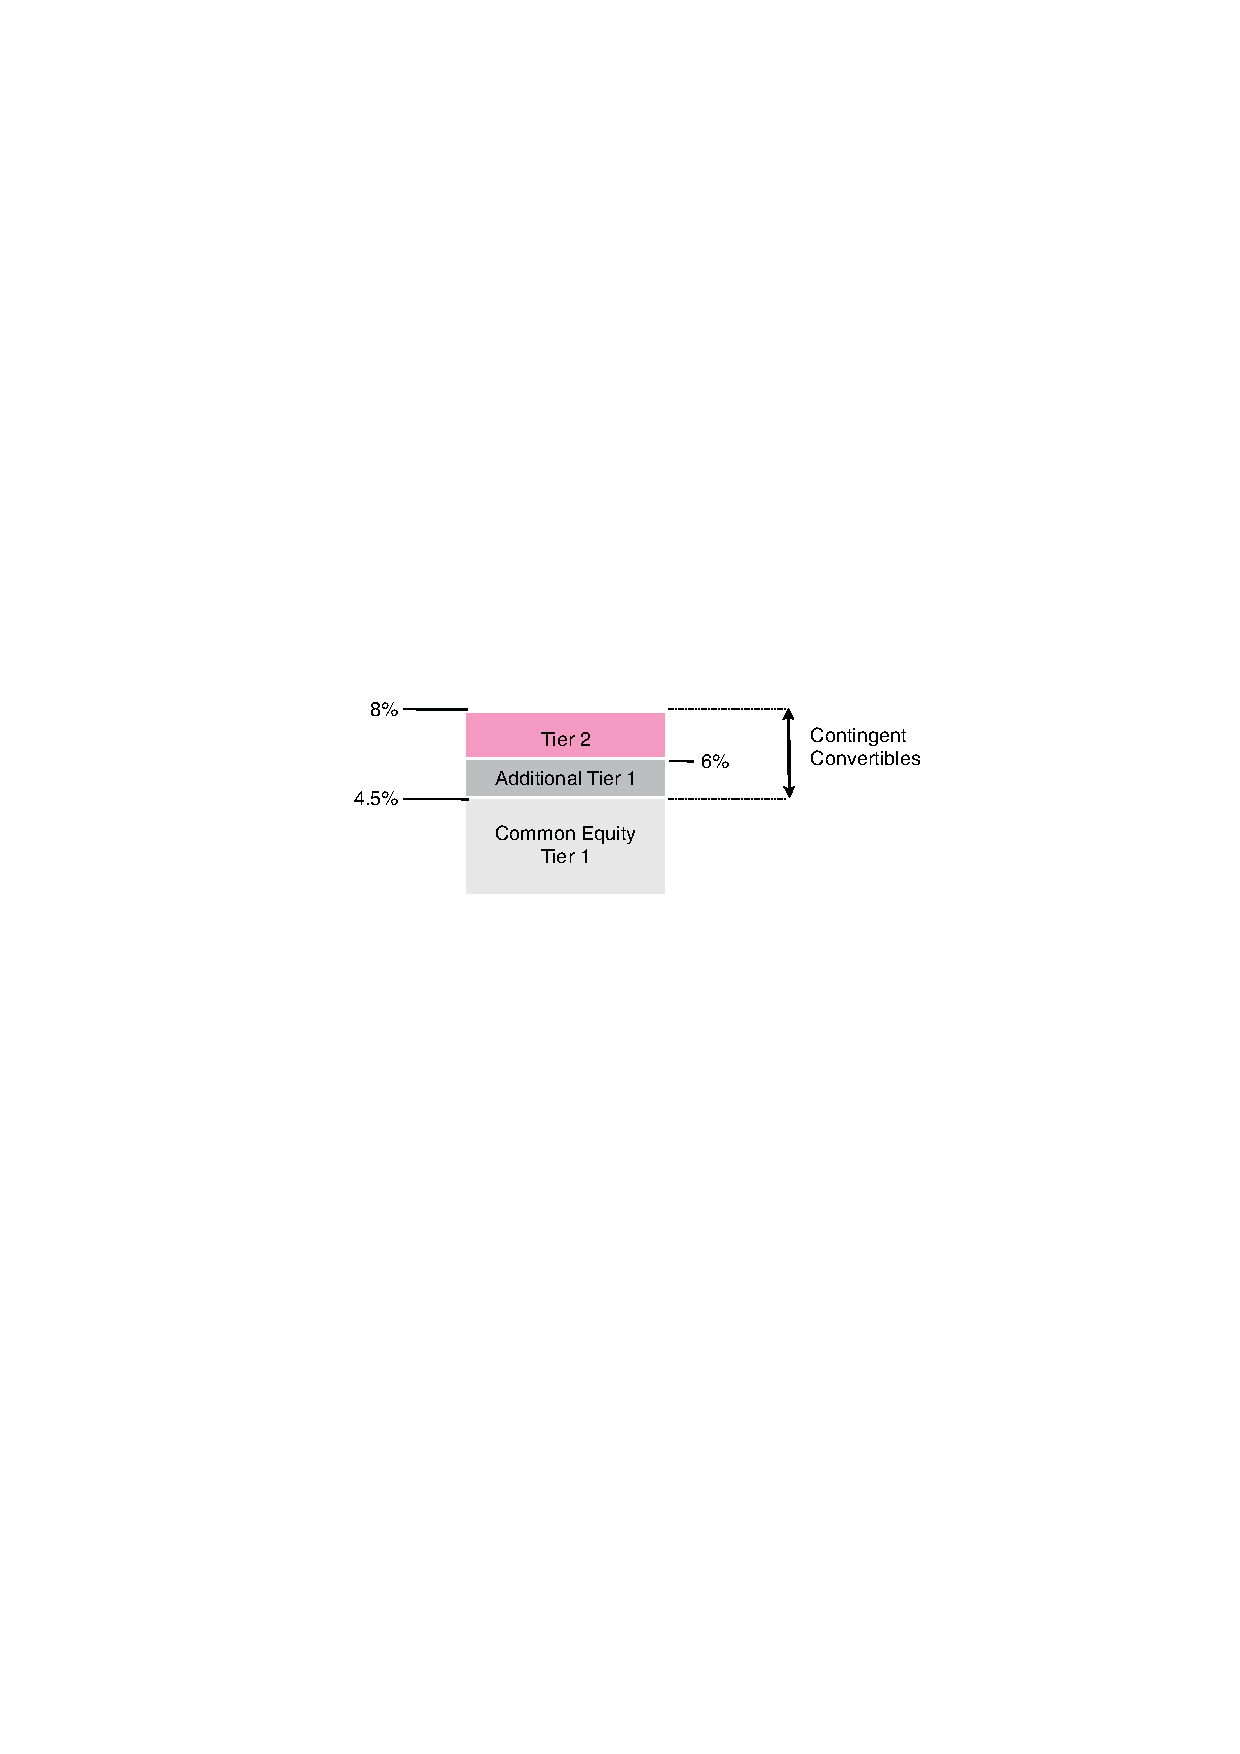
\includegraphics[trim=0.1cm 0.1cm 0.2cm 0.1cm, scale = 1]{media/basel3} \par
	\caption[CoCos under Basel III]{CoCos under Basel III \citep{de2011handbook}}
\end{figure}

\section{Payoff and Risk Profile}

\begin{figure}[ht]
	\centering
	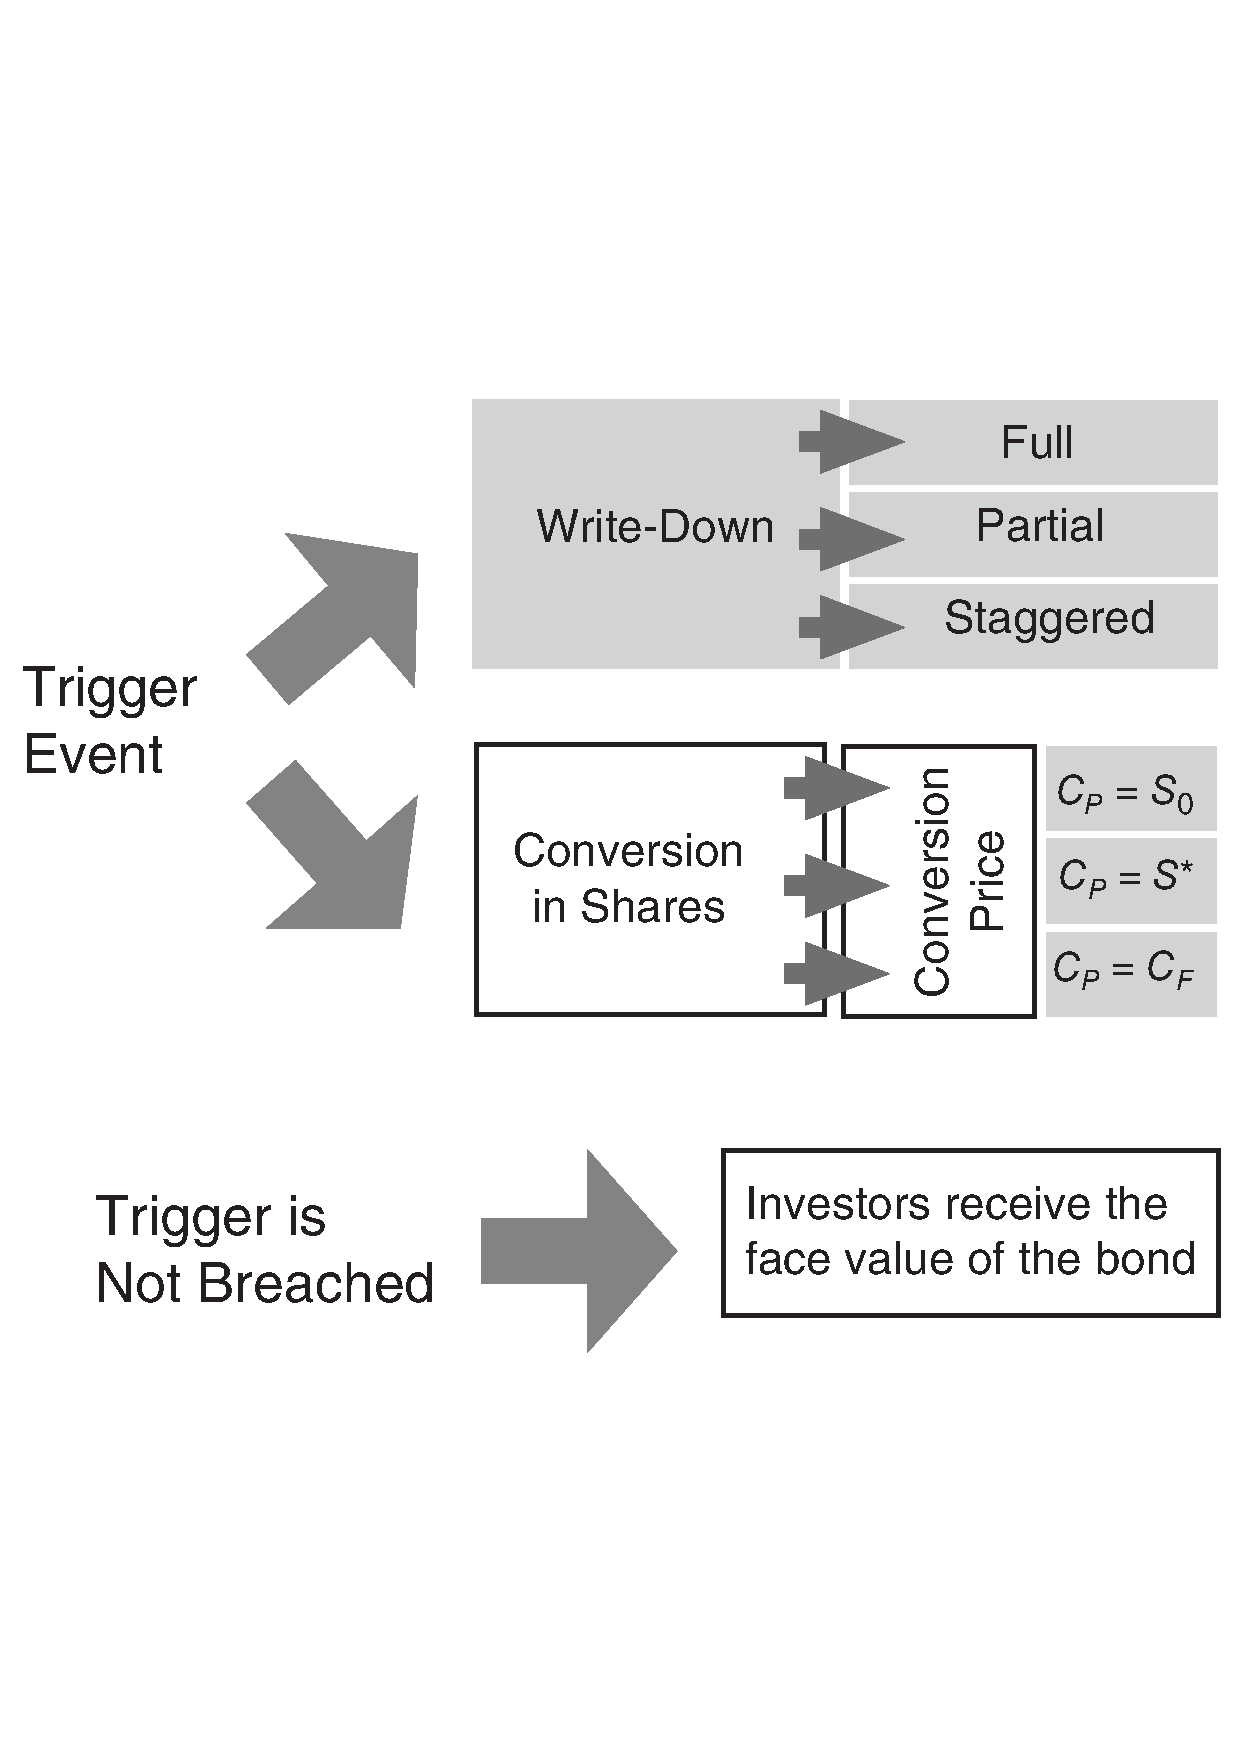
\includegraphics[trim=0.6cm 7.05cm 0.9cm 7cm, scale = 0.4]{media/anatomy} \par
	\caption[Anatomy of CoCos]{Anatomy of CoCos \citep{de2011handbook}}
\end{figure}

\section{Conversion Trigger}

\subsection{Market Trigger}

\subsection{Accounting Trigger}

\subsection{Regulatory Trigger}

\subsection{Multivariate Trigger}

\section{Conversion Details}

\subsection{Conversion Fraction}

\begin{itemize}
    \item conversion fraction $\alpha$
    \item face value $N$
    \item conversion amount $N \times \alpha$
    \item amount remaining in case of partial equity conversion $N \times (1-\alpha)$
\end{itemize}

\subsection{Conversion Price and Ratio}
%test
\begin{itemize}
    \item conversion rate $C_r$
    \item conversion price $C_p$
    \item recovery rate $R_{CoCo}$
    \item stock price at trigger event $S_T^{*}$
    \item loss attributable to CoCo holders $L_{CoCo}$
\end{itemize}

\begin{align}
    C_p &= \frac{\alpha N}{C_r}\\
    C_r &= \frac{\alpha N}{C_p}\\
    R_{CoCo} &= \frac{S_T^{*} }{C_p}\\
    L_{CoCo} &= N - ( 1 - R_{CoCo}) = N \left( 1 - \frac{S_T^{*}}{C_p} \right)\\
    P_T &= \begin{cases} (1 - \alpha) N + C_r S_T^{*} & \text{ if converted} \\ N & \text{if not converted} \end{cases}
\end{align}


\chapter{Theory of Pricing}

\section{Credit Derivative Approach}

\subsection{Intensity-based Approach}

\begin{align}
    p^* &= 1 - \exp\left(- \lambda_{Trigger} \times T\right)
\end{align}

\begin{align}
    s_{CoCo} &= \left(1 - R_{CoCo}\right) \times \lambda_{Trigger} = {Loss}_{CoCo} \times \lambda_{Trigger}
\end{align}

\begin{align}
    {Loss}_{CoCo} &= N - C_r \times S^* = N \left(1 - \dfrac{S^*}{C_P} \right)
\end{align}

\begin{align}
    R_{CoCo} &= \dfrac{S^*}{C_p}
\end{align}

\begin{align}
    p^* = \Phi\left( \dfrac{\log \left(\dfrac{S^*}{S}\right) - \mu T}{\sigma \sqrt{T}}\right) + \left(\dfrac{S^*}{S}\right)^{\dfrac{2 \mu}{\sigma^2}} \Phi\left( \dfrac{\log \left(\dfrac{S^*}{S}\right) + \mu T}{\sigma \sqrt{T}}\right)
\end{align}

\begin{align}
\lambda_{Trigger} &= - \dfrac{\log \left(1 - p^* \right)}{T}
\end{align}

\begin{align}
s_{CoCo} &= -\dfrac{\log \left(1 - p^*\right)}{T} \times \left( 1 - \dfrac{S^*}{C_p} \right)
\end{align}

\subsection{Application to CoCos}

\subsection{Data Requirements and Calibration}

\subsection{Pricing Example}

\section{Equity Derivative Approach}
Sources: \cite{erismann2015pricing}, \cite{de2011pricing}

\begin{align}
    P_T &= \mathbbm{1}_{\{ \tau > T \}} N +\left[ \left( 1 - \alpha \right) N + \dfrac{\alpha N}{C_p S^*} \right] \mathbbm{1}_{\{ \tau \leq T \}}\nonumber\\
    &= N + \left[ \dfrac{\alpha N}{C_p} S^* - \alpha N \right] \mathbbm{1}_{\{ \tau \leq T \}}\nonumber\\
    &= N + \left[ C_r S^* - \alpha N \right] \mathbbm{1}_{\{ \tau \leq T \}}\nonumber\\
    &= N + C_r \left[S^* - \dfrac{\alpha N}{C_r}\right] \mathbbm{1}_{\{ \tau \leq T \}}\nonumber\\
    &= N + C_r \left[ S^* - C_p \right] \mathbbm{1}_{\{ \tau \leq T \}}\nonumber
\end{align}

\begin{align}
    V^{ed}_t &= V^{cb}_t - V_{t_i}^{dibi} + V_t^{difwd}
\end{align}

\subsection{Corporate Bonds}
\begin{align}
    V^{cb}_t &= \sum^T_{i=t}c_i \exp\left(-r t_i\right) + N \exp\left[-r\left(T-t\right)\right]
\end{align}

\subsection{Binary Options}

\begin{align}
    V_t^{dibi}\left( c_i, S^*, t \right) &= \alpha \sum^k_{i=1} c_i \exp\left(-r t_i\right) \left[ \Phi\left(-x_{1i} + \sigma \sqrt{t_i}\right)\vphantom{\dfrac{S^*}{S}}\right.\nonumber\\
   &\qquad \left.\vphantom{\dfrac{S^*}{S_t}} +\left(\dfrac{S^*}{S_t}\right)^{2\lambda -2} \Phi\left(y_{1i} - \sigma \sqrt{t_i}\right) \right]
\end{align}

with 

\begin{align*}
x_{1i} &= \dfrac{\log \left( \dfrac{S_t}{S^*} \right)}{\sigma \sqrt{t_i}} + \lambda \sigma \sqrt{t_i}\\
y_{1i} &= \dfrac{\log \left( \dfrac{S^*}{S_t} \right)}{\sigma \sqrt{t_i}} + \lambda \sigma \sqrt{t_i}\\
\lambda &= \dfrac{r-q+\dfrac{\sigma^2}{2}}{\sigma^2}
\end{align*}

\subsection{Down-And-In Forward}

\begin{align}
    \max \left( S_T - K \right) \text{ if } \min_{0\leq t\leq T} \left( S_T \right) \leq S^*
\end{align}

\begin{align}
    \max \left( K - S_T \right) \text{ if } \min_{0\leq t\leq T} \left( S_T \right) \leq S^*
\end{align}

\begin{align}
V_t^{ dic }\left( S_t , S^* , K \right) &= S_t \exp \left[ - q \left(T-t\right) \right] \left( \dfrac{ S^* }{ S_t } \right) ^ { 2 \lambda } \Phi\left( y \right)\nonumber \\ 
&- K \exp \left[ - r \left(T-t\right) \right] \left( \dfrac{ S^* }{ S_t } \right) ^ { 2 \lambda - 2} \Phi \left( y - \sigma \sqrt{T-t} \right)
\end{align}

with 

\begin{align*}
K &= C_p\\
y &= \dfrac{\log\left( \dfrac{S^{* 2}}{S_t K} \right)}{\sigma \sqrt{T-t}} + \lambda \sigma \sqrt{T-t}\\
\lambda &= \dfrac{r-q+\dfrac{\sigma^2}{2}}{\sigma^2}
\end{align*}

\begin{align}
V_t^{dip}\left( S_t, S^*, K \right) &=  S_t \exp\left[ -q\left(T-t\right) \right] \left( \dfrac{S^*}{S_t} \right)^{2\lambda} \left[ \Phi\left(y\right) - \Phi\left(y_1 \right) \right]\nonumber\\
&- K \exp\left[ -r\left(T-t\right) \right] \left(\dfrac{S^*}{S_t}\right)^{2\lambda-2}\left[ \Phi\left( y- \sigma \sqrt{T-t} \right) -\Phi \left( y_1 - \sigma \sqrt{T} \right) \right] \nonumber\\
&+ K \exp\left[ - r \left(T-t\right) \right] \Phi \left( x_1 + \sigma \sqrt{T-t} \right)\nonumber\\
 &-S_t \exp\left[ -q \left(T-t\right) \right] \Phi\left( -x_1 \right)
\end{align}

with

\begin{align*}
x_1 &= \dfrac{\log\left(\dfrac{S_t}{S^*} \right)}{\sigma \sqrt{T-t}} + \lambda \sigma \sqrt{T-t}\\
y_1 &= \dfrac{\log\left(\dfrac{S^*}{S_t} \right)}{\sigma \sqrt{T-t}} + \lambda \sigma \sqrt{T-t}
\end{align*}

\begin{align}
\min\left( S_t\right) \leq S^* : P_T &= S_T -K = \max \left( S_T - K \right) -\max\left( K-S_T \right)
\end{align}

\begin{align}
\min\left( S_t \right) > S^* : P_T &= 0
\end{align}

\begin{align}
    V_t^{difwd} &= C_r \left[ S_t \exp\left[- q \left(T-t\right)\right]\left(\dfrac{S^*}{S_t}\right)^{2 \lambda} \Phi\left(y_1\right) \right.\nonumber\\
   &\qquad \left.\vphantom{\dfrac{S^*}{S_t}} - K \exp\left[- r \left(T-t\right)\right] \left(\dfrac{S^*}{S_t}\right)^{2 \lambda - 2} \Phi\left(y_1 - \sigma \sqrt{T-t}\right) \right.\nonumber\\
   &\qquad \left.\vphantom{\dfrac{S^*}{S_t}} - K \exp\left[- r \left(T-t\right)\right] \Phi\left(-x_1 - \sigma \sqrt{T-t}\right) \right.\nonumber\\
   &\qquad \left.\vphantom{\dfrac{S^*}{S_t}} + S_t \exp\left[- q \left(T-t\right)\right] \Phi\left(- x_1\right) \right] 
\end{align}

with 

\begin{align}
C_r &= \dfrac{\alpha N}{C_p}
\end{align}

\subsection{Data Requirements and Calibration}

\subsection{Pricing Example}

\section{Structural Approach}

\subsection{Synthetic Balance Sheet}

\subsection{Data Requirements and Calibration}

\subsection{Pricing Example}



 % Theory of Pricing
\chapter{Dynamics and Sensitivity Analysis}

\section{Credit Derivative Approach}

\section{Equity Derivative Approach}



\chapter{Case Study}\label{empiricalanalysis}

\section{Data Description}

\subsection{HSBC}

\section{Parametrization}

\section{Comparison}

\subsection{Qualitative Analysis}

\subsection{Quantitative Analysis}
\chapter{Conclusion}
The thesis has the objective to compare different valuation methods for CoCos. Three pricing approaches have been selected: the credit derivative approach, the equity derivative approach \citep{de2011pricing} and the structural approach \citep{pennacchi2010structural}. All approaches are brought into context to the current state of research. Apart from this, the paper provides comprehensive explanations of the theoretical concepts behind the valuation approaches.  Also, the models are applied consistently to a generic CoCo to understand their parametrization and implementation complexity. An application to a real-world CoCo of HSBC allows for further insights.\\

The first model, the credit derivative approach, is theoretically an elegant way to price CoCos. This is partly because the parametrization to market data is straightforward and fast calculations are guaranteed. However, conceptual weaknesses are detectable. A closer look into the model dynamics suggests that the model does not account for discontinuous returns. Hence, inherent tail risks are potentially underestimated. This seems to be confirmed by the fact that the estimated price of the generic CoCo is significantly higher than those of the equity derivative approach and the structural approach. Also, losses from canceled coupons of triggered CoCos are not taken into account in the valuation which might lead to an overestimation. From a practical viewpoint, the model does not inherit an equity spot process and therefore, equity risks cannot be determined. \citep{turfus2015cocos}\\

The equity derivative approach has strengths similar to those of the credit derivative approach. Though, they share conceptual flaws. They take the stock price at conversion as model input and not as stochastic output although it is very likely that equity jumps occur when the CoCo is triggered. \citep{turfus2015cocos} Furthermore, the equity derivative approach might underestimate the value of dividend payments to CoCo investors after the conversion has happened. One might also argue that credit risk calculations are not possible since the approach does not account for them. \citep{turfus2015cocos} \\

The structural approach complies very well with the hybrid nature of CoCos as it attempts to model the dynamics of the entire balance sheet. Tail risks are taken into consideration by factoring in a jump diffusion process to overcome the artificial simplification of continuous returns under a Black-Scholes setting. Though, several model inputs are necessary to apply the valuation approach to real world examples. An accurate estimation proves itself to be tough since certain parameters are not directly observable in the market or updated infrequently. The case study, however, reveals that a precise parameterization is indispensable. Also, good algorithm design skills are necessary to cut the calculation time of the Monte-Carlo simulation.

\begin{table}[H]
	\setlength{\extrarowheight}{2.5pt}
	\centering
	\begin{tabular}{lcccc}
		\toprule
			 & \textbf{CD} & \textbf{ED} & \textbf{SA}\\
		\midrule
			Price tracking accuracy & \cellcolor{red!20} low & \cellcolor{red!20} low & \cellcolor{yellow!20} medium\\
			Parametrization complexity & \cellcolor{green!20} low & \cellcolor{green!20} low & \cellcolor{red!20} high\\
			Calculation time & \cellcolor{green!20} low & \cellcolor{green!20} low & \cellcolor{red!20} high\\
		\bottomrule
	\end{tabular}
	\caption[Evaluation of pricing approaches with regard to three dimensions]{Evaluation of pricing approaches with regard to price tacking accuracy, parametrization complexity and calculation time}
	\label{table:evaluationtrigger}
\end{table}

Table \ref{table:evaluationtrigger} summarizes the results of the thesis. It becomes apparent that the parameterization is far more complicated for the structural approach compared to the other two approaches. Besides, the calculation time and associated cost are significantly higher for the structural approach. But the advantage is that the price tracking results are better over time. A shortcoming of all approaches is that they do not answer the question how confident they are about their own price estimates. As already mentioned, the applied pricing process might only be a heuristic that worked well for the HSBC CoCo in the observation period. Further empirical evidence should be conducted.








%\begin{itemize}
%\item include the notional in all models
%\item All models consider that at conversion the share price is equal to the trigger price
%\item But it is likely that jump occurs which potentially lessen the value of a CoCo
%\item downside of alll these models is that they do not lend themselves to prcing callable CoCo bonds, which are unfortunately common in practice
%\end{itemize}

%now enable appendix numbering format and include any appendices
\appendix
%\chapter{Sample Title}

\chapter{Code - Models} \label{creditderivativeapproach}
\section{Credit Derivative Approach} \label{creditderivativeapproach}

The following source code is an implementation of the Credit Derivative Approach \citep{de2011pricing} written in R.
 
\lstinputlisting[language=R]{code/CreditDerivativeApproach.R}

\section{Equity Derivative Approach} \label{equityderivativeapproach}

The following source code is an implementation of the Equity Derivative Approach \citep{de2011pricing} written in R.
 
\lstinputlisting[language=R]{code/EquityDerivativeApproach.R}

\section{Structural Approach} \label{structuralapproach}

The following source code is an implementation of the Structural Approach \citep{pennacchi2010structural} with support from \citet{codestructrural} in translating the source code of \citet{pennacchi2010structural} from GAUSS to R.
 
\lstinputlisting[language=R]{code/StructuralApproach.R}

\chapter{Code - Sensitivity Analyses}

\section{Credit Derivative Approach} \label{sensicredit}

The following source code is an implementation of the sensitivity analysis of the Credit Derivative Approach \citep{de2011pricing} written in R.
 
\lstinputlisting[language=R]{code/DiagramsCreditDerivativeApproach.R}

\section{Equity Derivative Approach} \label{sensiequity}

The following source code is an implementation of the sensitivity analysis of the Equity Derivative Approach \citep{de2011pricing} written in R.
 
\lstinputlisting[language=R]{code/DiagramsEquityDerivativeApproach.R}

\section{Structural Approach} \label{sensistructural}

The following source code is an implementation of the sensitivity analysis of the Structural Approach \citep{pennacchi2010structural} written in R.
 
\lstinputlisting[language=R]{code/DiagramsStructuralApproach.R}

\chapter{Code - Case Study}

\section{Parametrization - Structural Approach} \label{empirical}
The following source code is an implementation \citet{merton1974pricing} Model which is used to estimate the asset volatility written in R.
\lstinputlisting[language=R]{code/calibrateStructuralApproach.R}

\subsection{\citet{cox1985theory} Model}

The following source code is an implementation of the method as described by \citet{remillard2013statistical}. The method is used to calibrate the \citet{cox1985theory} model which is used for the structural approach pursuant to \citet{pennacchi2010structural} based on historical data. The software is an adaption of the source code as provided by \citet{calibrateCIR}.

\lstinputlisting[language=R]{code/estimateCIRParameter.R}\label{estimateCIRParameter}

\subsection{\citet{merton1974pricing} Model}
The following source code is an implementation of the \citet{merton1974pricing} model which is used to estimate the asset volatility. The code is written in R. Similar techniques are applied by \citet{stackoverflow2014code}.
\lstinputlisting[language=R]{code/estimateMertonParameter.R}\label{estimateMertonParameter}

\subsection{Jump-Diffusion Process}
The following source code is used to estimate the jump parameters after estimating the jump intensity. The code is written in R.
\lstinputlisting[language=R]{code/estimateJumpParameter.R}\label{estimateJumpsParameter}


 % Code Equity Derivative Approach

%next line adds the Bibliography to the contents page
\addcontentsline{toc}{chapter}{Bibliography}
%uncomment next line to change bibliography name to references
\renewcommand{\bibname}{References}
\bibliography{bibliography/refs}        %use a bibtex bibliography file refs.bib
\begin{acknowledgements}
plenty of waffle, plenty of waffle, plenty of waffle, plenty of waffle,
plenty of waffle, plenty of waffle, plenty of waffle, plenty of waffle.
\end{acknowledgements} 
%\begin{dedication}
This thesis is dedicated to my parents for their love and support.\\ 
Thank you!


\end{dedication}
\end{document}

